
\chapter{基于改进的Q-learning算法在直复营销中的研究}
普通的监督学习和非监督学习方法在处理代价敏感决策问题时,只能最大化单个事件的收益,不能考虑不同序列决策点之间的相互影响,因而不能很好的处理直复营销这种序贯决策问题。而强化学习方法在学习时,因为考虑到了序列延迟影响并以长期收益最大化作为优化目标,十分擅长处理序贯决策问题,所以本章选择使用强化学习的方法对该问题进行研究。首先使用强化学习的方法(Q-learning)对直复营销场景进行建模,然后针对营销点间的可变时间间隔问题,提出了针对Q-learning算法的状态值更新方法。并且,为了提高大数据集下模型训练的效率,基于Q-采样方法提出了改进的Q-采样方法。最后利用仿真环境进行评估试验,以此来验证所提方法的有效性。

\section{研究动机}
\subsection{直复营销与序贯决策}
如本文第一章所述,在直复营销场景中的每个营销时刻点,营销人员都需要根据客户的信息和之前的交互历史,做出应该对哪些客户进行营销的决策。在监督学习中,解决这个问题常用的方法有传统的分类算法和基于代价敏感的改进分类算法,然而这些算法都仅仅只考虑到了最大化单个独立决策事件的收益,并不能保证在一段时间上的长期收益最大化,这与直复营销最终所追求的目标不符。

直复营销是一个序贯决策过程,即随着时间的推移,营销人员需要不断地做出营销决策,并且以追求长期收益最大化作为目标。所以,在制定营销决策的时候,营销人员不仅需要考虑到每个决策行为的成本和其(即时)收益之间的关系,而且还要考虑到时间序列上不同决策点之间的相互影响。

考虑如下情景:在制定某次的营销决策时,营销人员发现,如果对某位客户进行营销的话,其产生的估计收益会大于营销成本,那么此时就不会对这位客户进行营销。然而,营销人员应该意识到,即使该客户在此次营销下不会产生即时的利润,但正是这一次的营销可能会有助于增加该客户在之后的营销中所产生的利润,甚至该利润值会很大。所以,营销人员在进行营销决策时,有时候需要牺牲即时收益以获得长期收益最大化。反之亦然,如果频繁地对某一位高质量用户发送营销信息,会降低该客户所能产生的期望收益,因为每一位客户在一段时间内消费能力是有限的。

\subsection{强化学习}
因为强化学习在学习过程中考虑到了序列中奖赏信号的延迟影响,并且以累积奖赏最大化作为学习目标。所以通过这种学习方式可以很好的处理直复营销决策中不同决策点之间的相互影响,进而达到长期收益最大化的目标,因此文献\citep{pednault2002sequential,archak2010budget,boutilier2016budget}等提出使用强化学习的思想来解决直复营销决策问题。但是,在上述相关工作中,以下问题仍然没有得到有效解决:在不定期营销场景中,各营销决策点之间的时间间隔是不确定的,所以就会给奖赏信号带来一定的噪声影响,从而影响了值函数的学习。另外,在实际应用中,随着数据规模的不断攀升,值函数的更新速度也会变慢。

本章针对以上两个问题进行分析,提出了相应的改进方法,以更好的解决直复营销问题。首先,利用马尔科夫决策过程,将直复营销问题建模为一个强化学习问题,并给出Q-learning算法解决该问题的框架;然后,为了解决营销决策点之间的可变时间间隔给奖赏信号带来的噪声影响问题,提出了基于可变时间间隔的Q-learning更新算法;最后,为了适应大批量数据的学习任务,在Q-采样的基础上,提出一种改进的Q-采样方法,以提高值函数的更新速度。

\section{改进的Q-learning算法在直复营销中的建模}
在本节中,首先使用Q-learning算法对直复营销场景进行建模,构建一个可以解决营销决策问题的模型框架。然后,针对不定期营销决策中的可变时间间隔问题,对Q-learning中值函数更新方法进行改进。接着,为了解决大数据集下模型更新的效率问题,基于TD偏差并在Q-采样方法的基础上,提出一个改进的Q-采样方法。

\subsection{直复营销问题形式化描述}
在本文的第二章中提到,强化学习问题可以使用如下马尔可夫决策过程来进行描述:在任意给定的时间点上,假设环境处于某个状态,当Agent采取一个行为时,它会收到一个有限的奖赏,并且环境会相应的转移到下一个状态。在这一过程中,Agent以最大化累计奖赏作为行为选择的依据,且该奖赏通常是以累计折扣的形式表示。

同样地,在使用强化学习解决直复营销问题之前,首先要使用马尔科夫决策过程对直复营销问题进行形式化的描述:在某一时刻$t$,客户的状态为$S_{t}$,如果营销人员对其采取了营销行为$A_{t}$,那么该客户的状态会根据一定的转移概率转移到下一状态$S_{t+1}$,并且客户会产生一定的奖赏信息$R_{t}$。以上这个过程始终贯穿于客户和营销人员的营销交互之中,那么,可以使用$\{<S_{t},A_{t},R_{t}>\}_{t=1}^{\infty}$三元组来表示每一次的营销事件。
其中,客户的状态$S_{t}$可以使用客户在该时刻所具有的特征信息来表示,比如文献\citep{tkachenko2015autonomous}中提到的Recency-Frequency-Monetary(最近交易时间、交易频率和交易金额)等,不同的营销行为$A_{t}$代表企业不同类型的营销方式,客户在反馈中所产生的奖赏信息$R_{t}$是指该客户产生的净利润,也就是说,强化学习在直复营销中是通过最大化每个客户生命周期价值,进而来达到最大化企业长期收益的目的。

在强化学习模型的选择上,Q-learning算法($\ref{algo:algorithm_2}$)以其原理简单、实现方便的优点,在实际中得到广泛应用。所以,接下来本章将参考文献\citep{,pednault2002sequential}中的基于函数逼近的批强化学习方法,给出Q-learning在直复营销问题中的模型框架。

\subsection{基于Q-learing的模型构建}
在传统的Q-learning算法中,值函数其实是一个表格,其索引是状态或者状态行为对,值迭代更新实际上就是这张表格的迭代更新。所以,Q-learning算法存在一个假设是,问题的状态空间和行为空间不能太大。然而,在像直复营销这类复杂的现实问题中,为了合理准确的表示客户的状态信息,需要非常多的特征,其状态空间自然非常大,所以,这时使用表格的形式进行值函数表示并不现实。

如第二章所述,对于状态空间较大的问题可以通过函数逼近的方法进行值函数的评估。在强化学习的各类函数逼近方法中,基于非参数化函数逼近的方法虽然具有很好的表征能力,但是随着数据量的增多其计算量呈指数升高,所以,不适合直复营销这类含有大量训练数据的场景。而在参数化函数逼近方法中,基于非线性的逼近方法在逼近过程中存在着收敛困难的问题。所以,考虑使用参数化线性逼近的方法进行值函数的逼近。另外,在参数化线性逼近方法中,基于增量式学习方法在参数的更新过程随机性较大,尽管计算简单,但样本的利用效率不高,而基于批的更新方法尽管计算复杂,但是计算效率较高。所以,本节选择使用基于批更新的线性函数逼近方法。

\paragraph{分块线性函数逼近}
尽管线性逼近方法可以收敛到全局最优解,但是其的表征能力较弱,为了缓解这个问题,本节考虑使用分块逼近的思想以提高值函数的逼近精度:

Q值函数分块逼近模型:考虑具有连续状态空间$S=\{S_{j}|j \in \mathbb{R}\}$和离散行为空间$A=\{A_{i}\}_{i=1}^{K}$的强化学习问题,利用逼近模型$M$对该问题的Q值函数进行建模。其中,$M=\{M_{i},\cdots,M_{K}\}$,其中$K$为离散行为个数。每个离散行为对一个子模型,子模型间相互独立,称$M$为Q值函数分块逼近模型。子模型可以采用任意的结构模型,若$K$个子模型结构相同,则称$M$为同构分块逼近模型,否则称为异构分块逼近模型。

基于以上分块逼近的思想,本节利用多项式基函数构建一组同构的分块线性逼近模型$Q=\{Q_{i}\}_{i=1}^{K}$,其中$Q_{i}=\bm{\theta}_{i}^{T} \phi(s)$ ,$\phi(s)$为多项式基函数。

假设第$i$个行为的数据集为$D_{i}=\{<S_{i,1},V_{i,1}>, <S_{i,2}, V_{i,2}>, \cdots <S_{i,n_{i}},V_{i,n_{i}}>\}$,其中$n_{i}$为第$i$个行为所对应的样本数量,使用批更新方法就是找到最好的拟合函数$Q_{i}$,使的$LS(\bm{\theta}_{i})=\sum_{t=1}^{n_{i}}(V_{i,t}-Q_{i}(S_{i,t},\bm{\theta}_{i}))$,那么,可用线性最小二乘进行逼近:
\begin{equation}\label{pifangfa}
\begin{aligned}
\Delta \theta_{i} = \alpha_{i} \sum_{t=1}^{n_{i}}[V_{i}-\bm{\theta}^{T} \phi(S_{i,t})] \phi(S_{i,t})
\end{aligned}
\end{equation}

\begin{algorithm}[htbp]
\small
\SetAlgoLined
\SetKwRepeat{Repeat}{repeat}{until} 
\KwData{折扣因子$\gamma$,最大迭代次数$P$,多项式次数$M$,原始总样本$D=\{e_{i}|i=1,\cdots,I\}$,$e_{i}=\{<S_{i,j}, A_{i,j}, R_{i,j}>|j=1,\cdots,l_{i}\}$,($D$表示样本集合,$e_{i}$表示第$j$个情节,$l_{i}$表示$e_{i}$的长度)}
\KwResult{输出最终的逼近模型:$Q^{(P)}$}

\For{all $e_{i} \in D$}{
	初始化第$i$个情节的数据:$D_{i}^{(0)}=\{<S_{i,j}, A_{i,j}, R_{i,j}>|j=1,\cdots,l_{i}\}$\;
}
整合所有情节的数据,生成总样本集合:$D^{(0)}=\cup_{i=1,\cdots,I} D_{i}^{(0)}$\;
将总样本集合$D^{(0)}$,按照行为标签ID$(A_{i,j}) \in \{1,2,\cdots, K \}$分发到各子模型的样本集合中,并利用分块线性函数更新公式$\eqref{pifangfa}$更新模型:$Q^{(0)}=\{Q_{i}^{(0)}\}_{i=1}^{K}$\;
\For{$p=1$ \KwTo $P$}{
	\For{all $e_{i} \in D$}{
		\For{$j$ \KwTo $l_{i}-1$}{
			更新状态行为值:\;
			$v_{i,j}^{(p)}=Q^{(p-1)}(S_{i,j},A_{i,j}) + \alpha^{(p)} (R_{i,j} + \gamma \max_{a} Q^{(p-1)}(S_{i,j+1},a)-Q^{(p-1)}(S_{i,j},A_{i,j}))$\;
		}
		更新第$i$个情节的样本:$D_{i}^{(p)}=\{<S_{i,j}, A_{i,j}, v_{i,j}^{(p)}>|j=1,\cdots,l_{i}-1\}$\;
	}
	整合所有情节的数据,生成总样本集合。$D^{(p)}=\cup_{i=1,\cdots,I}D_{i}^{(p)}$\;
	将总样本集合$D^{(p)}$,按照行为标签ID$(A_{i,j}) \in \{1,2,\cdots, K \}$分发到各子模型的样本集合中,并利用分块线性函数更新公式$\eqref{pifangfa}$更新模型:$Q^{(p)}=\{Q_{i}^{(p)}\}_{i=1}^{K}$\;
}
\caption{基于Q-learning的直复营销模型}
\label{algo:SVR+Q}
\end{algorithm}

\paragraph{模型的更新}
在传统的Q-learning算法中,还存在另一个假设,就是Agent可以与环境进行在线的交互。然而,像在直复营销这类复杂的现实应用中,构建这样的在线交互环境在很难的。为了解决这个问题,通常采用批强化学习\citep{lange2012batch}的方法进行解决,批强化学习是强化学习的一种形式,即Agent采取的行为、环境状态发生的转移都不以在线的方式进行,而是使用代表先前经验的大量静态训练数据进行离线的学习,通过这种方式可以反应现实生活应用中的真实情况。其中,训练数据由状态向量、动作值以及奖赏值所组成的三元组来构成。

结合以上批强化学习方法和分块线性函数逼近模型,可以得到用于解决直复营销问题的Q-learning算法框架,如$\ref{algo:SVR+Q}$所示。

在$\ref{algo:SVR+Q}$中,按照批强化学习的训练方法,将训练数据集$D$分成$I$个情节(episode),每个情节由一系列事件(event)组成,每个事件包含状态$s$、行为$a$和奖赏$r$。在每条情节数据中,保持了事件原有的出现顺序,以这种方式来重现真实的交互的过程。

在第一轮迭代中,首先初始化每个情节中的数据,整合成总样本集合$D^{(0)}$,然后按照总样本集合中行为标签值的不同划分$K$子样本集合,再利用分块线性逼近模型的更新公式$\eqref{pifangfa}$对奖赏值进行逼近,以此作为初步的估计Q值函数。在第二轮及之后的迭代过程中,根据上一次的估计值函数,利用Q值函数的更新公式,更新每个情节中每一个事件的状态行为值。当每一轮训练结束后,就将更新后的样本情节进行整合,形成总样本集合$D^{(p)}$,并按照行为标签值的不同划分$K$子样本集合,然后再利用分块线性逼近模型的更新公式$\eqref{pifangfa}$进行值函数的更新。当所有轮数迭代完毕后,输出最终的Q值函数。另外,对算法中学习率$\alpha$的选取,通常设置为$\alpha=\frac{1}{K}$,目的是让学习的步伐随着迭代次数的增加而不断减小。

\subsection{可变时间间隔问题}
在标准马尔科夫决策过程中,假设每个决策点之间的时间间隔是固定的,所以,如果在时刻$t=0$后接收到的奖赏序列为$\{R_{0}, R_{1},\cdots\}$,那么采用折扣累积奖赏的方式计算回报可用公式$\eqref{seq:reward_3}$来表示:
\begin{equation}\label{seq:reward_3}
G=\sum_{t=0}^{\infty}\gamma^{t}R_{t}
\end{equation}
式$\eqref{seq:reward_3}$中,$G$为回报,$\gamma<1$,为折扣因子。

但是,在不定期直复营销过程中,各个营销决策点之间的时间间隔是不确定的,有的间隔时间比较长,有的间隔时间比较短,那么不同时间间隔内所产生的奖赏对回报$G$的影响程度也是不同的。如图$\ref{fig:2_ad_process_}$所示,序列1是一条固定时间间隔的序列,序列2是一条可变时间间隔的序列,序列下面的第一行表示时间点,第二行表示该时间点所获得的奖赏,为了方便比较,假设序列1和序列2在每个时间点的获得的奖赏是相同的。以$t_{1}$时刻为例,序列1和序列2在$t_{1}$时刻虽然获得了相同的奖赏,但是其时间间隔$t_{1}-t_{0}$是不同的,那么,奖赏值$R_{2}$对回报的贡献自然也是不同的。而公式$\eqref{seq:reward_3}$计算累积奖赏的方法,只考虑到了序列上决策点的先后顺序,而忽略了时间间隔问题,因此如果序列2使用公式$\eqref{seq:reward_3}$计算回报,就会因为时间间隔问题而带来一定的噪声影响。
\begin{figure}[htbp]
\centering
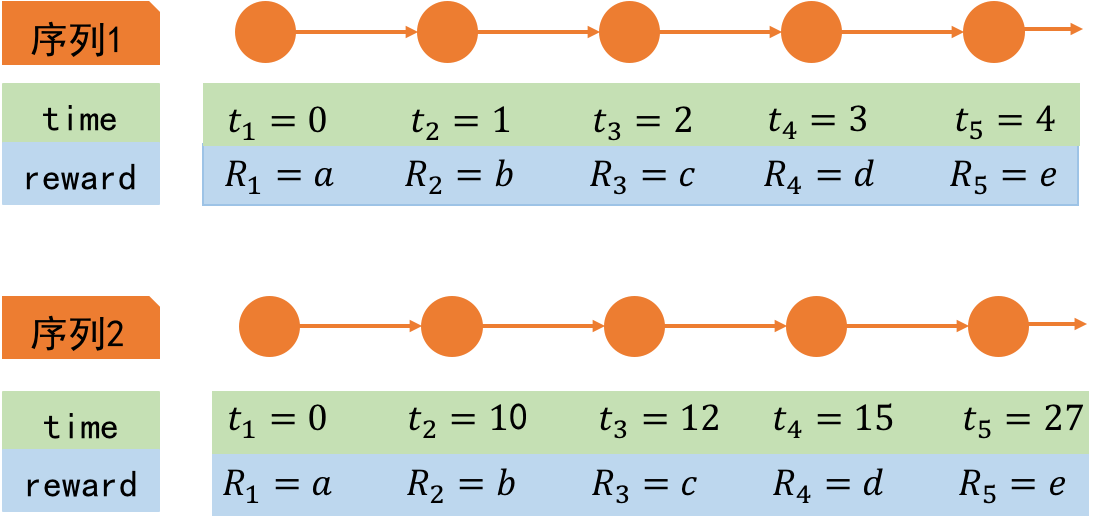
\includegraphics[width=0.8\textwidth]{2_ad_process_}
\caption{固定时间间隔和可变时间间隔序列}
\label{fig:2_ad_process_}
\end{figure}

和标准的马尔科夫决策过程相比,在带有可变时间间隔的马尔科夫决策过程中,每次的交互事件都会被标记上时间。假设整个马尔科夫决策过程是从$t_{1}=0$时刻开始的,并且初始状态为$S_{1}$,之后agent重复的采取行为,便会得到一系列的由行为、状态、奖赏以及时间组成的四元组$\{<S_{i},A_{i},R_{i},t_{i}>\}_{i=1}^{\infty}$,其中$t_{i}$就是第$i$个事件发生的时间。那么,在计算累积折扣奖赏时,折扣因子就被定义为关于时间的函数,如式\eqref{seq:r}所示:
\begin{equation}\label{seq:r}
\begin{aligned}
G=\sum_{i=1}^{\infty} \gamma^{t_{i}}R_{i}
\end{aligned}
\end{equation}

对应到算法$\ref{algo:SVR+Q}$中,如果将第$i$个情节的第$j$个事件和$j-1$个事件的时间差记为:$\triangle t_{i,j} = t_{i,j}-t_{i,j-1}$。那么,利用第5行对奖赏值$R_{i,j}$进行逼近后(作为初始的Q值函数),第10的更新公式可表示为:
\begin{equation}\label{seq:r1}
\begin{aligned}
v_{i,j}^{(p)}&=Q^{(p-1)}(S_{i,j},A_{i,j}) \\
&+  \alpha^{(p)} (R_{i,j} + \gamma^{\triangle t_{i,j+1}} \max_{a} Q^{(p-1)}(S_{i,j+1},a)-Q^{(p-1)}(S_{i,j},A_{i,j}))\\
&=(1-\alpha^{(p)})Q^{(p-1)}(S_{i,j},A_{i,j}) + \alpha^{(p)} (R_{i,j} + \gamma^{\triangle t_{i,j+1}} \max_{a} Q^{(p-1)}(S_{i,j+1,},a)\;
\end{aligned}
\end{equation}

\begin{equation}\label{seq:r_5}
\begin{aligned}
Z^{(p)}_{i,j}=(1-\alpha^{(p)})Z^{(p-1)}_{i,j}+\alpha^{(p)}(\triangle t_{i,j} + \gamma^{\triangle t_{i,j+1}} \cdot Z^{(p-1)}_{i,j+1})\;
\end{aligned}
\end{equation}

\begin{algorithm}[htbp]
\small
\SetAlgoLined
\SetKwRepeat{Repeat}{repeat}{until} 
\KwData{折扣因子$\gamma$,多项式次数$M$,最大迭代次数$P$,原始样本$D=\{e_{i}|i=1,\cdots,I\}$,$e_{i}=\{<S_{i,j}, A_{i,j}, R_{i,j}, t_{i,j}>|j=1,\cdots,l_{i}\}$,($D_{i}$表示第$i$个渠道的样本,$e_{i,j}$表示第$i$个渠道第$j$个情节,$l_{i,j}$为$e_{i,j}$的长度)}

\KwResult{输出最终的逼近模型:$Q^{(P)}$}

\For{all $e_{i} \in D$}{
	$\triangle t_{i,1}=1$\;
	\For{$j=2$ \KwTo $l_{i}$}{

		计算时间间隔,$\triangle t_{i,j}=t_{i,j}-t_{i,j-1}$\;
	}
}
\For{all $e_{i} \in D$}{
	\For{$j=1$ \KwTo $l_{i}-1$}{
		初始的标准化因子:$Z^{(0)}_{i,j}=\triangle t_{i,j}$\;
		初始的状态值:$v^{(0)}_{i,j} = R_{i,j}$\;
		将初始的状态值使用标准化因子进行标准化:$D_{i}^{(0)}=\{<S_{i,j}, A_{i,j}, \frac{v^{(0)}_{i,j}}{Z^{(0)}_{i,j}}>|j=1,\cdots,l_{i}\}$\;
	}
}

同算法$\ref{algo:SVR+Q}$中第4行到第5行\;

\For{$p=1$ \KwTo $P$}{
	\For{all $e_{i} \in D$}{
		\For{$j=1$ \KwTo $l_{i}-1$}{
			更新状态行为值\;
			$v_{i,j}^{(p)}=(1-\alpha^{(p)})Q^{(p-1)}(S_{i,j},A_{i,j}) \cdot \triangle  Z_{i,j}^{(p-1)} 
			+ \alpha^{(p)} (R_{i,j} + \gamma^{\triangle t_{i,j+1}} \max_{a} Q^{(p-1)}(S_{i,j+1,},a) \cdot \triangle  Z_{i,j+1}^{(p-1)} )$\;
			更新标准化因子\;
			$Z^{(p)}_{i,j}=(1-\alpha^{(p)})Z^{(p-1)}_{i,j}+\alpha^{(p)}(\triangle t_{i,j+1} + \gamma^{\triangle t_{i,j}} \cdot Z^{(p-1)}_{i,j+1})$\;
		}
		更新第$i$个情节的样本:$D_{i}^{(p)}=\{<S_{i,j}, A_{i,j}, \frac{v_{i,j}^{(p)}}{Z^{(p)}_{i,j}}>|j=1,\cdots,l_{i}-1\}$\;
	}
	同算法$\ref{algo:SVR+Q}$中第14行到第15行\;
}
输出最终的Q值函数$Q^{(P)} = Q^{(P)} \cdot Z^{(P)}$\;
\caption{基于可变时间间隔的Q-learning算法}
\label{algo:RBF-SVR-Q-t}
\end{algorithm}

由公式\eqref{seq:r}可以,获得奖赏$R_{i,j}$的时间间隔是不同的,所以如果直接使用原始奖赏值$R_{i,j}$进行Q值函数的逼近并应用在公式\eqref{seq:r1}中,就会因为可变时间间隔的影响,造成值函数更新不准确的问题。所以,一个自然的想法是,将时间间隔$\triangle t_{i,j}$内获得的奖赏值进行均值标准化,然后再使用标准化后的值进行值函数的更新。均值标准化的公式如\eqref{seq:r_1}所示:
\begin{equation}\label{seq:r_1}
\begin{aligned}
R_{i, j}^{'}=\frac{R_{i,j}}{t_{i,j}-t_{j-1}}=\frac{R_{i,j}}{\triangle t_{i,j}}
\end{aligned}
\end{equation}

那么,此时算法$\ref{algo:SVR+Q}$第10行的更新公式就可以按照如下式\eqref{seq:r_2}的方式进行更新:
\begin{equation}\label{seq:r_2}
\begin{aligned}
v_{i,j}^{(p)}=&(1-\alpha^{(p)})Q^{(p-1)}(S_{i,j},A_{i,j}) \cdot \triangle t_{i,j} \\
&+ \alpha^{(p)} (R_{i,j} + \gamma^{\triangle t_{i,j+1}} \max_{a} Q^{(p-1)}(S_{i,j+1,},a) \cdot \triangle t_{i,j+1})
\end{aligned}
\end{equation}

接着,按照算法$\ref{algo:SVR+Q}$第11行进行情节样本的更新:
\begin{equation}\label{seq:r_3}
\begin{aligned}
D_{i}^{(p)}=\{<S_{i,j}, A_{i,j}, \frac{v_{i,j}^{(p)}}{\triangle t_{i,j}}>|j=1,\cdots,l_{i}-1\}\;
\end{aligned}
\end{equation}

从公式\eqref{seq:r_2}中可以看出,随着迭代次数的增加,$v_{i,j}$在不断变化,而$\triangle t_{i,j}$是始终不变的,如果按照公式\eqref{seq:r_3}更新情节样本的方式($\frac{v_{i,j}^{(p)}}{\triangle t_{i,j}}$),会带来一定的偏差。所以,在值函数的更新过程中,应该仿照$v_{i,j}$的更新方式进行$\triangle t_{i,j}$的更新。针对这个问题,本文基于时间间隔构建一个标准化因子$Z_{i,j}$,并仿照$v_{i,j}$的更新方式进行标准化因子的更新,以解决之前更新方式所带来的偏差影响。标准化因子的更新方式可表示为式\eqref{seq:r_5}


由此,可以得到基于可变时间间隔的Q-learning算法如$\ref{algo:RBF-SVR-Q-t}$所示,记为IntervalQ。其中,第1行到第6行进行时间间隔的计算,第7行到第13行进行标准化因子以及样本的的初始化,第19行进行状态行为值的更新,第21行进行归一化因子的更新,第23进行情节样本的更新。

\subsection{改进的采样方法}
在直复营销等类似的现实应用场景中,数据量非常大,如果将全部样本都导入模型中进行训练,将必然会加重模型的训练负担,另外,Q值函数的更新也会消耗很多的时间。所以,为了解决以上问题,应该采取有效的采样方法来加快模型的训练和更新速度。

在强化学习中,常用的采样方法有随机采样法和Q-采样法,随机采样法,就是在每次从数据集中取情节的时候(如算法$\ref{algo:RBF-SVR-Q-t}$中,第7行和第16行),并不是取所有的情节,而是随机选取部分的情节,这种随机采样方法虽然可以减轻模型的训练和值函数的更新时间,但是由于随机性较高,导致采样后的数据质量并不高,因而会影响最后值函数的逼近效果。Q-采样法,是在随机采样的基础上提出的,当进行Q值函数的更新的时候,不是每个情节中所有事件都会被选择用于值函数的更新,而只有那么利用当前的估计Q值函数,可以在下一个状态中取得最佳行为的状态才能被选择。即在算法$\ref{algo:RBF-SVR-Q-t}$的第11到21行替换成如下算法$\ref{algo:SVR+Q_}$的语句:

\begin{algorithm}[htbp]
\small
\SetAlgoLined
\SetKwIF{If}{ElseIf}{Else}{if}{then}{else if}{else}{endif}
从数据集合$D$中随机采样一个样本子集,$R^{(p)}$\;
\For{all $e_{i} \in R^{(p)}$}{
	\For{$j$ \KwTo $l_{i}-1$}{
		\If{$Q^{(p-1)}(S_{i,j+1},A_{i,j+1})=\max_{a}Q^{(p-1)}(S_{i,j+1},a)$}{
			$v_{i,j}^{(p)}=(1-\alpha^{(p)})Q^{(p-1)}(S_{i,j},A_{i,j}) \cdot Z_{i,j}^{(p-1)} 
			+ \alpha^{(p)} (R_{i,j} + \gamma^{\triangle t_{i,j+1}} \max_{a} Q^{(p-1)}(S_{i,j+1,},a) \cdot  Z_{i,j+1}^{(p-1)} )$\;
			$Z^{(p)}_{i,j}=(1-\alpha^{(p)})Z^{(p-1)}_{i,j}+\alpha^{(p)}(\triangle t_{i,j+1} + \gamma^{\triangle t_{i,j}} \cdot Z^{(p-1)}_{i,j+1})$\;
		}
		更新第$i$个情节的样本:$D_{i}^{(p)}=D_{i}^{(p)} \cup \{<S_{i,j}, A_{i,j}, \frac{v_{i,j}^{(p)}}{Z^{(p)}_{i,j}}>\}$\;
	}
}
\caption{基于Q采样的算法}
\label{algo:SVR+Q_}
\end{algorithm}

但是,通过Q采样的方法进行采样后的样本仍然很大,而且,即使选择了在下一状态中可以达到最佳行为的当前状态,但是该状态并不一定会有很高的学习效率。

考虑在本文第二章中,由公式$\eqref{shijiachafen}$计算出的$t$时刻的时间差分TD:$\delta_{t}$,应用在算法$\ref{algo:SVR+Q_}$的Q值函数中,可表示为式$\eqref{shijiachafenq}$:
\begin{equation}\label{shijiachafenq}
\begin{aligned}
&\delta_{i,j}=R_{i,j} + \gamma^{\triangle t_{i,j+1}} Q^{(p-1)}(S_{i,j+1}, a) \cdot Z_{i,j+1}^{(p-1)}  - Q^{(p-1)}(S_{i,j},A_{i,j}) \cdot Z_{i,j}^{(p-1)} \\
&\text{其中,} a=\argmax_{a} (Q^{(p-1)}(S_{i,j+1},a) \cdot Z_{i,j+1}^{(p-1)})
\end{aligned}
\end{equation}

式$\eqref{shijiachafenq}$中,$R_{i,j} + \gamma^{\triangle t_{i,j+1}} Q^{(p-1)}(S_{i,j+1}, a) \cdot Z_{i,j+1}^{(p-1)}$称为TD目标,即值函数逼近的目标值。如果TD偏差$\delta_{t}$越大,说明该状态处的值函数$Q^{(p-1)}(S_{i,j},A_{i,j}) \cdot Z_{i,j}^{(p-1)}$与TD目标目标的差距越大,进一步可以说明agent的更新量越大,因此在该处的学习效率就越高。所以,本文的想法是,在进行Q-采样的时候,可以根据TD偏差的大小再一次进行有选择的采样。具体地,当使用Q采样算法$\ref{algo:SVR+Q_}$第4行条件进行初步选择后,设定一个固定的阈值$\eta$,然后使用公式$\eqref{shijiachafenq}$再一次进行选择,只选择TD偏差大于$\eta$的样本进行更新。所以,依据这个想法修改算法$\ref{algo:SVR+Q_}$就可以得到基于TD的Q采样方法如$\ref{algo:SVR+Q_2}$所示。

\begin{algorithm}[htbp]
\small
\SetAlgoLined
\SetKwIF{If}{ElseIf}{Else}{if}{then}{else if}{else}{endif}
\KwData{增加一个TD偏差阈值$\eta$}
从数据集合$D$中随机采样一个样本子集,$R^{(p)}$\;
\For{all $e_{i} \in R_{k}$}{
	\For{$j$ \KwTo $l_{i}-1$}{
		\If{$Q^{(p-1)}(S_{i,j+1},A_{i,j+1})=\max_{a}Q^{(p-1)}(S_{i,j+1},a)$ $\bm{And}$
			利用公式$\eqref{shijiachafenq}$计算的$\delta_{i,j} \geqslant$  $\eta$
		}{
			$v_{i,j}^{(p)}=(1-\alpha^{(p)})Q^{(p-1)}(S_{i,j},A_{i,j}) \cdot Z_{i,j}^{(p-1)} 
			+ \alpha^{(p)} (R_{i,j+1} + \gamma^{\triangle t_{i,j}} \max_{a} Q^{(p-1)}(S_{i,j+1,},a) \cdot  Z_{i,j+1}^{(p-1)} )$\;
			$Z^{(p)}_{i,j}=(1-\alpha^{(p)})Z^{(p-1)}_{i,j}+\alpha^{(p)}(\triangle t_{i,j} + \gamma^{\triangle t_{i,j+1}} \cdot Z^{(p-1)}_{i,j+1})$\;
		}
		更新第$i$个情节的样本:$D_{i}^{(p)}=D_{i}^{(p)} \cup \{<S_{i,j}, A_{i,j}, \frac{v_{i,j}^{(p)}}{Z^{(p)}_{i,j}}>\}$\;
	}
}
\caption{基于TD偏差的Q采样算法}
\label{algo:SVR+Q_2}
\end{algorithm}

\section{仿真实验}
本节,借助直复营销场景中的直邮营销数据集进行模型的训练,并通过仿真的方法进行模型的评估。首先,对实验中所使用的数据集进行介绍,并详细说明所选择的客户特征信息;然后,介绍本实验中的仿真环境构建以及评估方法;接着介绍本章试验所用的模型以及试验设置信息;最后,从模型的长期收益、所产生的策略行为以及不同采样方法等三方面进行试验评估并对结果进行分析。

\subsection{数据集}
本章选择使用UCI数据库中关于直邮营销著名的公开数据集KDD-CUP 1998\footnote{https://kdd.ics.uci.edu/databases/kddcup98/kddcup98.html}。该数据集有两个用途,一方面,利用数据集中的数据进行模型的训练,生成营销策略。另一方面,利用该数据集构建马尔科夫决策过程的仿真模型,然后利用这个仿真模型进行仿真试验,以评估不同模型所产生的营销策略。

\paragraph{数据集背景}
直邮营销是直复营销中最早的、也是最为经典的应用场景,它通过对目标客户以邮寄的方式达到营销宣传的目的。KDD-CUP 1998数据集是由美国非盈利组织PVA(Paralyzed Veterans of America)收集的,该组织通过直邮的方式向潜在捐助者发布捐助活动信息以
筹集资金,为有脊髓损伤疾病的美国退伍军人提供援助。

该数据集是在PVA直邮捐助营销过程中所产生的信息组成。共包括了95412名捐助者的信息,每条信息包括捐助者的个人基本信息(共计361维)以及在两年间所进行的22次募捐活动的历史营销纪录(共120维),这些记录包括:PVA是否向该捐助者进行了邮寄营销、该捐助者是否对这次的邮寄营销产生了反馈、如果产生了反馈该捐助者捐助了多少钱等信息,另外邮寄的时间以及捐助者的反馈时间都是可获得的,从数据中发现,相邻两个营销点的时间间隔为0-3个月不等。
% 其中23个捐助活动中又含有11种不同类型的邮件。
有关该数据集的其它描述信息可在UCI网站上获得。

\paragraph{特征选择}
首先,需要确定模型中的数据结构。在算法$\ref{algo:RBF-SVR-Q-t}$中,数据是以情节(episode)的形式存在的,每个情节内有包含一系列有序的事件(event),每个事件是由状态,行为、奖赏和时间所构成的四元组。因此,在KDD-CUP 1998数据集中,可以将每个捐助者产生的22次营销数据看作一个情节,每次营销看作一个事件。那么,每个捐助者就对应一个情节,每个情节里有22个事件,且22个事件是按照真实的营销时间有序排开的。特别地,每个事件里包括该捐助者此时的状态,PVA对其采取的营销行为、此次营销捐助的金额以及该时间发生的时间。


\begin{table}[htbp]
  \centering
  \caption{捐助者特征的选取}
  \label{tab:obser_donors}
  \begin{tabular}{lll}
    \toprule
      序号 & 特征 & 描述 \\
    \midrule
      1 & age & 捐助者的年龄 \\
      2 &income & 捐助者的收入 \\
      3 &ngiftall & 捐助者的捐助的次数 \\
      4 &numprom & 向该捐者发送直邮营销的次数 \\
      5 &frequency & 该捐助者捐助的频率:numgiftall / numprom \\
      6 &ramntall & 捐助的总金额 \\
      7 &recency & 距离上次捐助的时间 \\
      8 &promrecency & 距离上次发送直邮营销的时间\\
      9 &timelag & 第一次直邮营销和第一次捐助的时间\\
      10 &recencyratio & recency / timelag\\
	  11 &promrecratio & promrecency / timelag\\
      12 &nrecproms6 & 之前六个月里,给该捐者者发送直邮营销的次数\\
      13 &nrecgifts6 & 之前六个月里,捐助者捐助的次数\\
      14 &totrecamt6 & 之前六个月里,捐助者捐助的金额之和\\ 
      15 &nrecproms3 & 之前六个月里,给该捐者者发送直邮营销的次数\\
      16 &nrecgifts3 & 之前六个月里,捐助者捐助的次数\\
      17 &totrecamt3 & 之前六个月里,捐助者捐助的金额之和\\            	  
	  18 &action & PVA的营销类型,0表示未进行,1表示已进行\\
	  19 &money &  捐助的金额\\
    \bottomrule
  \end{tabular}
\end{table}

为了能够准确描述捐助者在每一次营销活动时的状态,需要借助专家领域知识,选取高效的特征。本节参考文献\citep{pednault2002sequential}中的特征选取方法,进行了捐助者特征的提取。具体地,在KDD-CUP 1998数据集中针对每个捐助者的基本信息,本章只选择了年龄和收入两个指标。另外,根据根据数据集中的营销交互信息,生成了许多临时特征。如表~\ref{tab:obser_donors}所示。其中,第18条的action属性对应事件中的行为信息,第19条的money属性减去营销的成本就是对应事件中的奖赏信息,其余特征对应事件中的捐助者状态信息。特别地,为了更好的捕捉到捐助者的状态,本节使用了一个六个月时间的历史窗口来提取捐助者的近期的状态特征,那么,前六个月内的数据就被第一个历史窗口信息,所以,一个情节中22个事件中就只剩下了16个可以用于模型的训练之中了。


需要注意的是,表~\ref{tab:obser_donors}中的大部分捐助者的状态特征都无法从数据集中直接得到,而只能需要通过遍历数据库统计得到。比如,在数据集中,每个捐助者的numprom字段只有一个值,它表示的意思是最后一次营销(第22次)结束后向该捐者发送直邮营销的次数 ,那么我们为了得到在每一次营销时的捐助者信息,应该从后往前进行遍历,每当在直邮营销活动中发现PVA对该捐助者进行了邮寄,就进行减一操作。同样,对于ngiftall字段,每个捐助者也只有一个值,它表示的意思时最后一次营销结束后该捐助者捐助的次数,而我们为了得到每一次营销时的捐助者信息,应该从后往前进行遍历,每当在营销活动中发现该捐助者进行了捐助就进行减一操作。其他的特征也都需要进行类似的统计计算,以得到捐助者在每个营销点的状态信息。

\subsection{仿真环境及评估方法}
评估强化学习模型的好坏需要有稳定的仿真环境。目前,OPENAI提供了许多游戏的仿真环境开源库,科研人员可以通过其提供的API接口非常方便的调用这些仿真环境,来训练、测试自己模型,所以,这也是目前大多数强化学习的研究者选择在游戏领域进行研究的一个重要方面。然而,在其它的一些应用中,需要研究人员根据训练数据自己构建仿真环境。本节,针对KDD-CUP 1998数据集,按照文献\citep{pednault2002sequential}提供的方法,通过构建关于数据集的马尔科夫决策过程来搭建仿真环境,进而评价模型输出策略的好坏。

\paragraph{构建MDP模型}
构建马尔科夫决策过程主要由两个评估模型组成:第一个模型$P(s,a)$是用来预测捐助者的产生募捐反馈的响应概率,它是一个关于状态$s$和行为$a$的函数。第二个模型$A(s,a)$用来预测如果募捐者对此次募捐邮件产生了响应,会产生多少金额的募捐。其中,在本节的实验中模型$P(s,a)$和$A(s,a)$分别使用随机森林分类模型和随机森林回归模型进行构建。

如图$\ref{fig:simulation}$中间位置的“仿真环境模块”所示,当有了模型$P(s,a)$和$A(s,a)$就可以使用如下过程来构建马尔科夫决策过程,。

(1)给定状态$s$和行为$a$下的即时奖赏$R(s,a)$可以通过这两个模型得到:以$P(s,a)$的概率来掷一枚硬币,并以此来判断捐助者是否会产生反馈。即:出现正面的概率为$P(s,a)$表示捐助者会产生反馈,出现反面的概率为$1-P(s,a)$表示捐助者忽略掉了本次募捐邮件,不会产生任何反馈信息。如果没有出现反馈,那么捐助额为$0$,如果产生了反馈,那么用户的捐助金额为$A(s,a)$。即时奖赏$R(s,a)$等于捐助额减去邮寄的成本。

(2)状态转移方程也可以通过使用这两个模型计算每一个状态特征的变化情况而得到。比如:如果PVA采取的行动为1,numprom的值就会加1,否则保持不变;同样的,如果上述掷硬币的方式出现正面朝上,那么ngiftall的值就会加1,否则保持不变;有了这两个值(numprom,ngiftall),那么frequency的值也就可以计算出来了。类似的,其他状态特征也是通过这种方法计算的到的。

\begin{figure}[htbp]
\centering
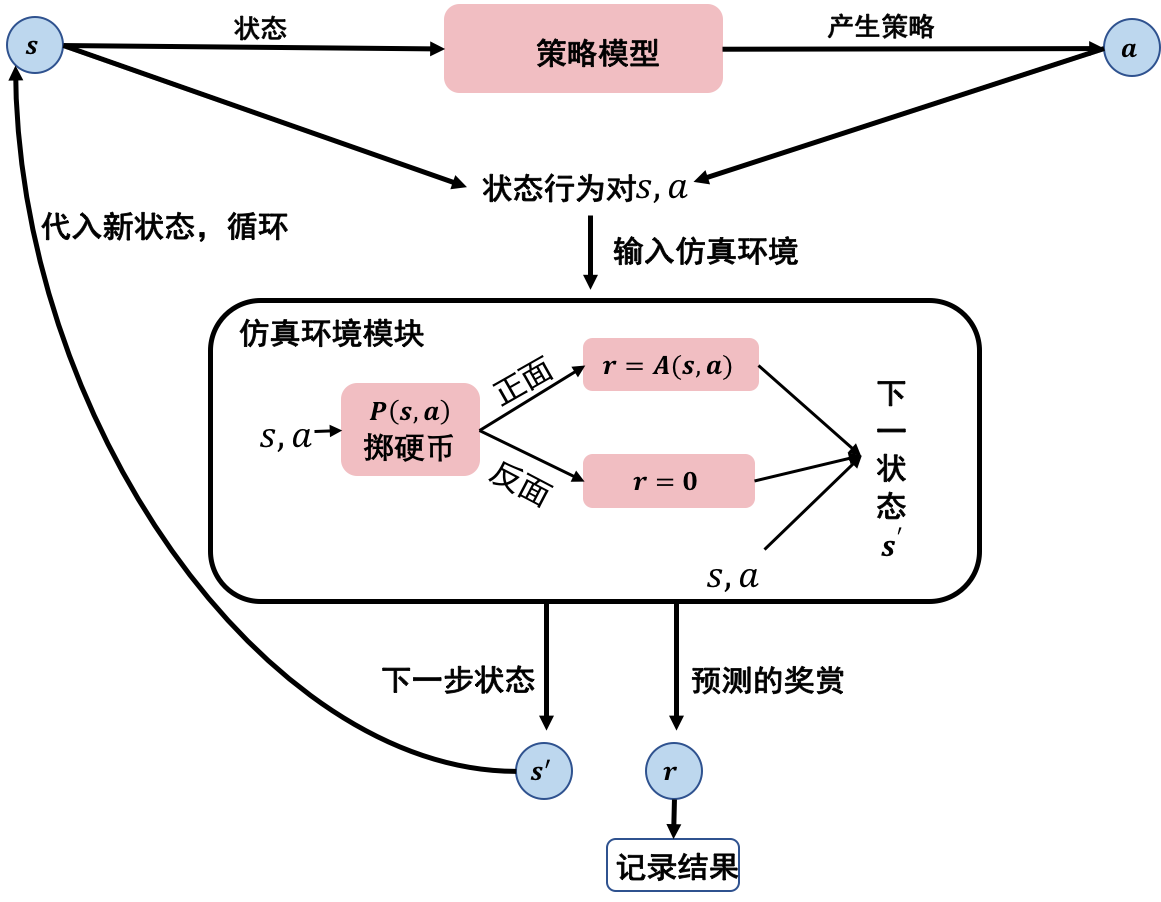
\includegraphics[width=0.75\textwidth]{simulation}
\caption{仿真评估实验流程图}
\label{fig:simulation}
\end{figure}

\paragraph{评估方法}
如图$\ref{fig:simulation}$所示,有了上述马尔科夫决策过程的模型和状态转移方程,就可以使用如下的方式来构建我们的评估实验。

(1)首先,随机选择一定数量规模(5000)的捐助者,并设置他们的初始状态。本实验中将所选择的捐助者的初始状态设置为第7次营销时的状态。

(2)然后,使用训练好的强化学习模型输出营销策略:对每个捐助者是否应该采取营销行为。

(3)最后,将状态$s$和策略行为$a$代入仿真环境中,使用模型$P(s,a)$和$A(s,a)$,可以得到预估的即时奖赏$r$以及下一时刻的状态$s^{'}$。记录这些得到信息,然后进入下一次的邮寄决策中。

就这样,按照上述的三个步骤,每循环一次就会模拟一次虚拟的直邮营销的过程。在本节实验中,重复循环了20次,就会得到了20次的虚拟直邮营销数据。

在文献\citep{pednault2002sequential}中作者提出,构建上述仿真环境的假设前提是认为募捐者的交互过程是一个马尔科夫决策过程,但是,在现实中这不一定是合适的。作者认为,像直复营销这种与人类行为有关的场景都过于复杂,使用简单的马尔科夫决策过程是无法较好的捕捉到环境的变化规律的,但是,我们使用这个仿真环境只是去评估我们的模型所产生的策略的好坏,只是在真实场景应用前的一个评估实验。所以,这种评估方法是可接受的,也是目前强化学习评估实验所普遍采用的方法。

\subsection{基准模型与实验设置}
\paragraph{基准模型}
本节共选择三个基准模型,其中包括:

(1)监督学习模型:为了比较监督学习模型和强化学习在序列决策上的优缺点,本节选择使用随机森林回归模型基于状态$s$和行为$a$来预测即时奖赏$r$,记为$\hat{R}(s,a)$。当模型训练好后,根据募捐者的状态$S_{t}$选择可以使的即时奖赏最大化的营销行为$A_{t}=\argmax_{a} \hat{R}(S_{t},a)$。

(2)batch Q-learning算法\citep{pednault2002sequential},以此来比较引入可变时间间隔因素后对模型策略效果的影响。

(3)Q-采样方法($\ref{algo:SVR+Q_}$),以此来评估改进的Q-采样方法的效果。

\paragraph{实验设置}
(1)每个试验运行5次,每次试验最大迭代次数为8,在每次迭代接受后进行模型策略的评估,并取5次试验在每一次迭代中的平均值作为最终的结果。如上文所述,评估样本规模为5000,他们的初值状态对应第7次营销活动时的状态。

(2)在所有的强化学习方法中,衰减因子设为$\gamma=0.9$,多项式次数为3。

(3)在使用随机森林构建时,通过网格搜索法确定:最大的弱学习器的个数为100个,决策树最大深度为25。

\subsection{仿真结果}
下面,本节将分别从模型的长期收益、模型的策略行为以及不同采样方法的效果对比等三方面展开模型的评估。具体地,在比较模型长期收益和模型的策略行为时,本节将基于可变时间间隔的Q-learning(IntervalQ)方法、batch Q-learning算法以及随机森林模型(监督学习方法)进行对比。然后,从样本采样数量、长期收益两方面来比较随机采样、Q采样方法以及本章所提的改进Q采样方法。

\paragraph{长期收益}
首先,考察IntervalQ模型,batch Q-learning模型以及SL模型在20个虚拟营销中的总收益。在本小节的实验中,每次试验选取10,000个情节(10,000个用户的交互记录)也就是160,000条事件数据进行训练,当每次迭代结束后利用仿真环境进行评估实验,输出20个虚拟营销的总利润。

\begin{table}[htbp]
\centering
\footnotesize
\caption{IntervalQ模型结果}
\label{tab:3result1}
\begin{tabular}{lccccccccccc}  
 \toprule
  迭代数 & 1&2 &3 &4 &5 &6 &7 &8\\
\midrule
  第一次 & 1&2 &3 &4 &5 &6 &7 &8\\
  第二次 & 1&2 &3 &4 &5 &6 &7 &8\\
  第三次 & 1&2 &3 &4 &5 &6 &7 &8\\
  第四次 & 1&2 &3 &4 &5 &6 &7 &8\\
  第五次 & 1&2 &3 &4 &5 &6 &7 &8\\
  平均值 & 1&2 &3 &4 &5 &6 &7 &8\\
  标准差 & 1&2 &3 &4 &5 &6 &7 &8\\
\bottomrule
\end{tabular}
\end{table}


图[]展示了IntervalQ和batch Q-learning模型这5次试验中每次迭代的平均收益值,其中第0次迭代表示使用线性多项式回归方法监督学习所产生的总收益,误差线表示五次试验中的总利润的标准误差,计算方法如下:
\begin{equation}\label{seq:shiyan_2}
\begin{aligned}
\sigma = \sqrt{\frac{\sum_{i=1}^{n}(F_{i}-\bar{F})^{2}/n-1}{n}}
\end{aligned}
\end{equation}

$\eqref{seq:shiyan_2}$中,$F_{i}$表示在第i次迭代中的总收益,$\bar{F}$表示5次迭代中的总收益。从图中可以清楚的看到,使用强化学习的方法在之后的迭代中总收益明显超过了监督学习的方法。从图中可以看出,IntervalQ和batch Q-learning比SL模型具有显著的长期收益,而且因为考虑到了可变时间间隔的影响,IntervalQ在第4轮迭代以后比batch Q-learningyou很好的表现。从模型的稳定性上看,提出的IntervalQ的稳定性也好于batch Q-learning算法

一方面证明强化学习的方法比监督学习的方法在序列化决策问题上会有更好的收益,另一方面期望证明基于可变时间间隔的ntervalQ模型在直复营销场景中比普通batch Q-learning模型有更好的表现。

\paragraph{策略的行为}
接着,考察以上三个模型得到的20个营销策略是如何变化的。图()显示了第10次迭代输出的20个营销活动中每次营销邮寄的人数。同样,在这个实验中,仍然选择5000个募捐者作为营销对象,从图中可以看出,通过IntervalQ和batch Q-learning算法在5个营销活动后有更好的成本控制能力,特别地,通过强化学习产生的营销策略可以看出,它最初邮寄给比较多的目标对象,等待观察回应,然后又再次尝试发给较多的目标对象,通过这种不断的尝试理解募捐者的交互行为,可以使的在序列决策上作出最优的策略。

进一步,本节考察随着营销时间的推移,每一次营销所产生的利润是如何变化的。图()显示了第10次迭代输出的20次营销策略的所获的利润。从图中,可以清楚的看出,强化学习方法产生的营销策略最初获得利润较低,但是在之后的营销活动中,其获得的利润在不断提升这表明考虑到长期影响的强化学习方法是以最大化长期价值为目标,而不是为了获得短暂的即时收益。

还要注意的是,尽管第二次营销期间所发送的邮件数量很少,但是仍然有很大的利润。这些利润代表了先前营销活动的延迟回应,所以,该利润被记录到了他们收到捐款的时间而不是进行营销的时间。所以,从这一方面也可以看出,为了可以准确的在马尔科夫决策过程中作出序列决策,应该考虑到延迟影响的信用分配问题。

\paragraph{采样方法比较}
最后,从输出策略的质量和采样的数据集大小来验证本节提出采样方法的有效性。图()展示了随着迭代次数的增大,不同采样方法所获得的长期利润。主要是将本章提出的改进Q采样方法和Q采样方法以及随机采样方法的对比。图()展示了随着迭代次数的变化,不同采样方法的采样规模是如何变化饿。在这三个实验中,使用了大小为10,000的情节数据集,其中每次迭代时又5,000个被随机抽样,也就是80,000个事件数据。从图中可以看出,改进的Q采样方法相比Q采样方法进一步降低了样本数量。

另外,比较这两幅图清楚地表明了所提出的抽样方法的优点。通过改进的Q采样方法,不仅不会因为减少样本而使的所获的长期利润变小,反而可以产生更多的收益,侧面反正了这种采样方法可以提高样本的的学习效率。因为该实验中的行为数只有两个,而在许多实际应用中,可能会有大量可能的行为可供选择。在这种情况下,人们可以期望在计算资源方面有相当大的节省。

\section{本章小结}
针对传统Q-learning算法在解决直复营销问题中的不足,本章从可变时间间隔和采样方法两方面进行改进。首先,给出直复营销在强化学习框架下的形式化描述以及基于Q-learning的算法模型,然后针对营销决策点之间存在的可变时间间隔问题,针对Q-learning算法进行改进,并改进值函数的更新方法。接着,针对Q-learning算法在处理大规模数据时的学习效率较低的问题,基于Q-采样的方法,提出了改进的Q-采样方法。最后,介绍仿真环境的构建方法,并利用仿真环境从模型的长期收益、策略行为的变化以及采样方法的效果等三个方面对所提算法进行评估并对结果进行分析,评估结果验证了所提算法的有效性。

